\subsection{Simulation}
\label{sec:simulation}
The model is tested with a step from $0$ to $47.8 Nm$, which correspond to a target q-current of $300 A $. At the start the load torque is set to $20 Nm$, and after $0.5 s$ it is increased to $40 Nm$. 

The three phase currents produced can be seen on figure \ref{fig:iabc}.

\begin{figure}[H]
	\centering
	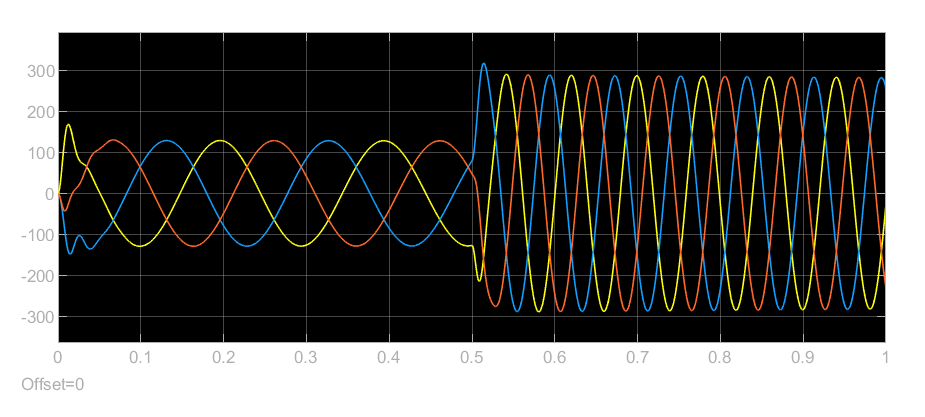
\includegraphics[width=0.7\linewidth]{pictures/control/iabc.eps}
	\caption{The ABC current from the motor model}
	\label{fig:iabc}
\end{figure}

As it is seen on figure \ref{fig:iabc}, the amplitude of the current increases when a bigger load is put on the motor. 
% A higher demand of current was expected when a bigger load is put on the motor. 

The d- and q-current can be seen on figure \ref{fig:idq}.

\begin{figure}[H]
	\centering
	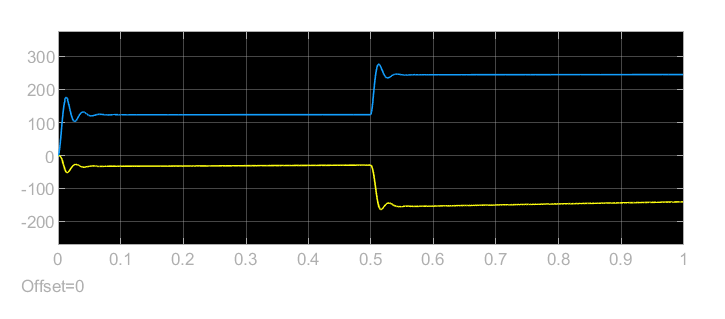
\includegraphics[width=0.7\linewidth]{pictures/control/idq.eps}
	\caption{The d- and q-current from the motor model. The yellow curve is the d-current and the blue curve is the q-current}
	\label{fig:idq}
\end{figure}

On figure \ref{fig:idq} it can be seen that the q-current is not going toward the set reference. It can also be seen that the d-current is very slowly going towards zero.

On the figure \ref{fig:speed} and \ref{fig:torque} the speed and the torque of the motor can be seen.

\begin{figure}[H]
	\centering
	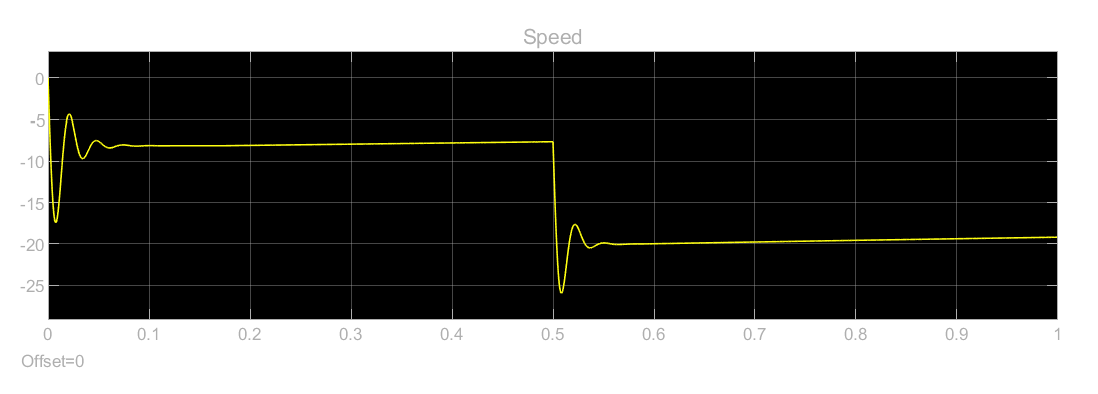
\includegraphics[width=0.7\linewidth]{pictures/control/speed.eps}
	\caption{The speed of the motor}
	\label{fig:speed}
\end{figure}

\begin{figure}[H]
	\centering
	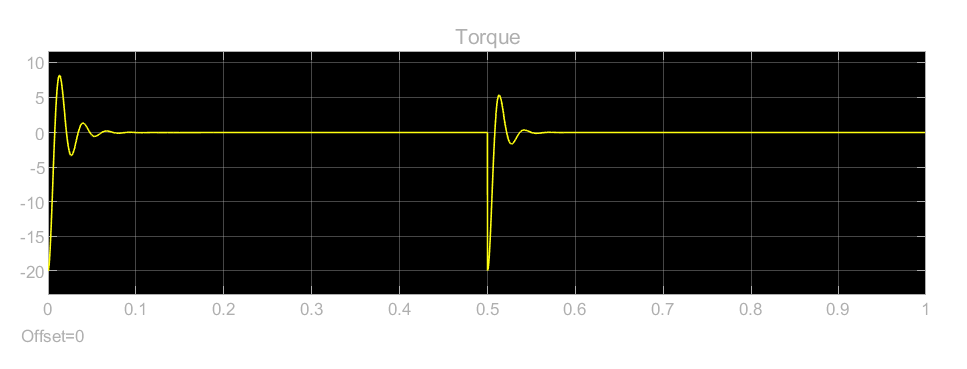
\includegraphics[width=0.7\linewidth]{pictures/control/torque.eps}
	\caption{The torque of the motor}
	\label{fig:torque}
\end{figure}

